\subsection{可度量化空间的仿紧性}

下述定理加强了第 1 号命题 2 的结果：

定理 4. 每个可度量化空间都是仿紧的。

该定理是下述四个引理的推论。

引理 3. 设 \(\Re = (U_{\alpha})_{\alpha \in A}\) 是可度量化空间 \(X\) 的一个开覆盖。则存在一个序列 \((\mathfrak{S}_n)\) ，它由 \(X\) 的开子集组成的局部有限族构成，使得 \(\mathfrak{S} = \bigcup \mathfrak{S}_n\) 是 \(X\) 的一个加细 \(\Re\) 的开覆盖。

设 \(d\) 是 \(\mathbf{X}\) 上与其拓扑相容的度量。对每个 \(\alpha \in \mathbf{A}\) 及每个整数 \(n\) ，令 \(\mathbf{F}_{n\alpha}\) 表示诸 \(x \in \mathbf{U}_{\alpha}\) 中满足 \(d(x, \mathbf{X} - \mathbf{U}_{\alpha}) \geqslant 2^{-n}\) 者所成的集。由于 \(\mathbf{X} - \mathbf{U}_{\alpha}\) 是闭集，我们有 \(\mathbf{U}_{\alpha} = \bigcup_{n} \mathbf{F}_{n\alpha}\) 。把集 \(\mathbf{A}\) 良序化；对每个 \(\alpha \in \mathbf{A}\) 及每个整数 \(n\) ，令 \(\mathbf{G}_{n\alpha}\) 为诸 \(x \in \mathbf{F}_{n\alpha}\) 中满足 \(x \notin \mathbf{F}_{n+1,\beta}\) （对一切 \(\beta < \alpha\) ）者所成的集，并令 \(\mathbf{V}_{n\alpha}\) 为诸 \(y \in \mathbf{X}\) 中满足 \(d(y, \mathbf{G}_{n\alpha}) - 2^{-n-3}\) 者所成的集。\(\mathbf{V}_{n\alpha}\) 显然是开集；另一方面，\(\mathbf{V}_{n\alpha} \subset \mathbf{U}_{\alpha}\) ，因为对每个 \(y \in \mathbf{V}_{n\alpha}\) 存在 \(x \in \mathbf{G}_{n\alpha}\) 使 \(d(x, y) \leqslant 2^{-n-1}\) ，而由 \(x \in \mathbf{F}_{n\alpha}\) ，我们有

\[
d (y, \mathrm{X} - \mathrm{U} _ {\alpha}) \geqslant d (x, \mathrm{X} - \mathrm{U} _ {\alpha}) - d (x, y) \geqslant 2 ^ {- n - 1},
\]

从而 \(y \in \mathbf{U}_{\alpha}\) 。再者，对每个 \(x \in \mathbf{X}\) ，设 \(\alpha\) 是 \(\mathbf{A}\) 中使 \(x \in \mathbf{U}_{\alpha}\) 的最小指标；则存在整数 \(n\) 使 \(x \in \mathrm{F}_{n\alpha}\) ，而由 \(\alpha\) 的定义推出 \(x \in \mathrm{G}_{n\alpha}\) ，从而 \(x \in \mathrm{V}_{n\alpha}\) 。这表明，若令 \(\mathfrak{S}_n = (\mathrm{V}_{n\alpha})_{\alpha \in \mathbf{A}}\) ，则 \(\mathfrak{S} = \bigcup_{n} \mathfrak{S}_n\) 便是 X 的一个开

覆盖，且加细 \(\Re\) ；于是剩下要证明的是，诸族 \(\mathfrak{S}_n\) 中的每一个都局部有限。为此我们先证明不等式 \(d(\mathrm{G}_{n\alpha}, \mathrm{G}_{n\beta}) \geqslant 2^{-n-1}\) 对 \(\alpha \neq \beta\) 成立。设 \(\beta < \alpha\) ；那么若 \(x \in \mathrm{G}_{n\alpha}\) 且 \(y \in \mathrm{F}_{n\beta}\) ，则由定义有 \(x \notin \mathrm{F}_{n+1, \beta}\) ，因而 \(d(x, \mathrm{X} - \mathrm{U}_{\beta}) < 2^{-n-1}\) ，而 \(d(y, \mathrm{X} - \mathrm{U}_{\beta}) \geqslant 2^{-n}\) ，于是 \(d(x, y) \geqslant 2^{-n-1}\) ；由于 \(\mathrm{G}_{n\beta} \subset \mathrm{F}_{n\beta}\) ，断言得证。由此，利用 \(\mathrm{V}_{n\alpha}\) 与 \(\mathrm{V}_{n\beta}\) 的定义立即推出 \(d(\mathrm{V}_{n\alpha}, \mathrm{V}_{n\beta}) \geqslant 2^{-n-2}\) 。由最后这个不等式推出：对每个 \(z \in \mathrm{X}\) ，以 \(z\) 为中心、\(2^{-n-3}\) 为半径的开球至多与族 \(\mathfrak{S}_n\) 中的一个集相交；因而 \(\mathfrak{S}_n\) 是局部有限族，证明完毕。

引理 4. 设 \((\mathfrak{S}_n)\) 是拓扑空间 \(\mathbf{X}\) 中开集的局部有限族所成的序列，使得

\[
\mathfrak {S} = \bigcup_ {n} \mathfrak {S} _ {n}
\]

是 X 的覆盖。则存在 X 的一个局部有限（但不一定开的）覆盖 B ，它加细 S 。

设 \(\mathbf{E}_n\) 是 \(\mathbf{X}\) 中的开集，即 \(\mathfrak{S}_n\) 中所有集的并；

令 \(U_{n}\) 表示 \(\bigcup_{k=1}^{n}E_{k}\) ，并令 \(A_{n}\) 表示 \(U_{n}-U_{n-1}\) （约定 \(U_{0}=\varnothing\) ）。考察形如 \(V\cap A_{n}\) 的子集所成的集 B ，其中 \(V\in S_{n}\) 而 n 为任意整数；我们来证明 B 满足引理的条件。对每个 \(x\in X\) 存在整数 n 使 \(x\in A_{n}\) ，因为诸 \(A_{n}\) 构成 X 的一个分划；于是 \(x\in E_{n}\) ，从而存在 \(V\in S_{n}\) 使 \(x\in V\) ；故 \(x\in V\cap A_{n}\) ，这就证明了 B 是 X 的覆盖。显然，此覆盖加细 S 。另一方面，对每个 \(x\in X\) 存在整数 n 使 \(x\in U_{n}\) ；由于 \(U_{n}\) 是开集而诸 \(S_{m}\) 是局部有限族，故对每个 m 存在 x 的邻域 \(W_{m}\) ，它含于 \(U_{n}\) 且只与 \(S_{m}\) 中有限多个集相交；因而 x 的邻域 \(W=\bigcap_{m=1}^{n}W_{m}\) 只与 B 中有限多个集相交，因为 \(W\cap A_{p}=\varnothing\) 对 p\textgreater n 成立。于是 B 局部有限，引理 4 得证。

引理 5. 设 X 是正则空间，使得对 X 的每个开覆盖 R ，存在 X 的一个（不一定开的）局部有限覆盖 A 加细 R 。则对 X 的每个开覆盖 R ，存在 X 的一个局部有限闭覆盖 F 加细 R 。

设 \(\mathfrak{R}\) 是 X 的任一开覆盖。对每个 \(x \in \mathbf{X}\) ，存在开集 \(\mathbf{U} \in \mathfrak{R}\) ，它包含 \(x\) ，从而（由于 X 正则）存在一个开邻域 \(\mathbf{V}_x\) （它包含 \(x\) ），使 \(\overline{\mathbf{V}}_x \subset \mathbf{U}\) 。族 \(\mathfrak{B}\) 由诸 \(\mathbf{V}_x\) 组成，它是 X 的一个开覆盖，故由假设存在一个局部有限覆盖 \(\mathfrak{B}\) 加细 \(\mathfrak{B}\) 。设 \(\mathfrak{F}\) 为 \(\mathfrak{B}\) 中诸集的闭包所成的族。由于覆盖 \(\mathfrak{B}'\) （由诸 \(\overline{\mathbf{V}}_x\) 组成）比 \(\mathfrak{R}\) 更细，而 \(\mathfrak{F}\) 又比 \(\mathfrak{B}'\) 更细，故 \(\mathfrak{F}\) 是 X 的一个加细 \(\mathfrak{R}\) 的闭覆盖。此外 \(\mathfrak{F}\) 还是局部有限的，因为若一个开集不与集 \(\mathbf{B} \in \mathfrak{B}\) 相交，则它也不与其闭包 \(\overline{\mathbf{B}}\) 相交。

引理 6. 设 X 是豪斯多夫空间，使得对 X 的任一开覆盖 R ，存在 X 的一个加细 R 的局部有限闭覆盖 F 。则 X 是仿紧的。

设 \(\mathfrak{R}\) 是 X 的任一开覆盖。我们要证明存在 X 的一个加细 \(\mathfrak{R}\) 的局部有限开覆盖。设 \(\mathfrak{A}\) 是 X 的一个加细 \(\mathfrak{R}\) 的局部有限覆盖（闭与否均可）；对每个 \(x \in \mathbf{X}\) ，设 \(W_x\) 是 \(x\) 的一个开邻域，它只与 \(\mathfrak{A}\) 中有限多个集相交。族 \(\mathfrak{B}\) 由诸集 \(W_x\) 组成，它是 X 的一个开覆盖。设 \(\mathfrak{F}\) 是 X 的一个加细 \(\mathfrak{B}\) 的局部有限闭覆盖。对每个 \(A \in \mathfrak{A}\) ，设 \(U_A\) 是 \(\mathfrak{R}\) 中包含 A 的一个集，并设 \(C_A\) 为诸集 \(F \in \mathfrak{F}\) 中满足 \(A \cap F = \emptyset\) 者的并。由于 \(\mathfrak{F}\) 局部有限，\(C_A\) 在 X 中闭（第 I 章，§ 1，第 6 号，命题 4），因而 \(A' = U_A \cap (X - C_A)\) 是开集。由于 \(A \cap C_A = \emptyset\) 且 \(A \subset U_A\) ，故 \(A \subset A'\) ，而族 \(\mathfrak{A}'\) （由诸集 \(A'\) 组成，其中 A 取遍 \(\mathfrak{A}\) ）是 X 的一个开覆盖；再者，由于 \(A' \subset U_A \in \mathfrak{R}\) ，\(\mathfrak{A}'\) 加细 \(\mathfrak{R}\) 。剩下要证明 \(\mathfrak{A}'\) 局部有限。对每个 \(x \in X\) 存在 \(x\) 的一个邻域 T ，它只与 \(\mathfrak{F}\) 中有限多个集、设为 \(F_1, \ldots, F_n\) 相交。由于每个 \(F_i\) 含于形如 \(W_{y_i}\) 的一个集中，按定义 \(F_i\) 只与 \(\mathfrak{A}\) 中有限多个集相交；设 \(A_{ij} (i \leqslant j \leqslant s_i)\) 就是这些集。若 A 是 \(\mathfrak{A}\) 中异于诸 \(A_{ij} (i \leqslant i \leqslant n, i \leqslant j \leqslant s_i)\) 的一个集，则由诸定义推出 \(A'\) 不与任何 \(F_i\) 相交，因而不与 \(T \subset \bigcup_{i=1}^{n} F_i\) 相交。这就完成了引理 6 与定理 4 的证明。

\section{贝尔空间}

\subsection{无处稠密集}

定义 1. 拓扑空间 X 的子集 A 称为无处稠密的，如果它的闭包没有内点。

等价地，A 在 X 中无处稠密当且仅当 A 的外部在 X 中稠密。

闭集 A 无处稠密当且仅当它没有内点，亦即当且仅当它与自己的边界相重合。任一子集 A 无处稠密当且仅当 A 的闭包无处稠密。无处稠密集的每个子集都无处稠密。

例。1) X 的空子集是无处稠密的。在豪斯多夫空间 X 中，由单独一点组成的集是无处稠密的，当且仅当该点在 X 中不是孤立点。稠密子集决不会是无处稠密的（除非 \(X = \varnothing\) ）。

\begin{enumerate}
\def\labelenumi{\arabic{enumi})}
\setcounter{enumi}{1}
\item
开集或闭集的边界总是无处稠密的。
\item
在空间 \(\mathbf{R}^n\) 中，每个维数 \(p < n\) 的线性子空间都是无处稠密集（第 VI 章，§ 1，第 4 号，命题 2）。
\end{enumerate}

注。任意子集的边界未必是无处稠密的：例如，若 A 与 \(\mathbb{C}\) A 都是稠密集，则 A 的边界是整个空间。

命题 1. 有限多个无处稠密集的并是无处稠密的。

只需证明两个无处稠密集 A、B 的并是无处稠密的，并且不失一般性可设 A 与 B 都是闭集。于是该命题等价于说两个稠密开集 CA、CB 的交是稠密的。现设 U 是非空开集，则 \(U \cap CA\) 是开集且非空，从而

\[
\left(\mathrm{U} \cap \mathbb {C A}\right) \cap \mathbb {C B} = \mathrm{U} \cap \left(\mathbb {C A} \cap \mathbb {C B}\right)
\]

是开集且非空。

设 Y 是拓扑空间 X 的子空间。Y 的子空间 A 称为相对于 Y 无处稠密的，如果 A 作为拓扑空间 Y 的子集来看是无处稠密的。

命题 2. 设 Y 是拓扑空间 X 的子空间，A 是 Y 的子集。若 A 相对于 Y 无处稠密，则 A 相对于 X 无处稠密。反之，若 Y 在 X 中开且 A 相对于 X 无处稠密，则 A 相对于 Y 无处稠密。

设 A 相对于 Y 无处稠密。若 A 在 X 中的闭包 \(\overline{A}\) 含有一个非空开集 U ，则 \(U \cap A\) 非空（由闭包的定义）；于是 \(U \cap Y\) 是相对于 Y 的非空开集，且含于 A 相对于 Y 的闭包 \(\overline{A} \cap Y\) 之中，这与假设相矛盾。

现设 Y 在 X 中开，且 \(A \subset Y\) 相对于 X 无处稠密。若 U 在 Y 中开且非空，则 U 在 X 中开，从而含有一个在 X 中（因而在 Y 中更是）开的非空集 V ，且 V 不与 A 相交；故 A 相对于 Y 无处稠密。

若 Y 在 X 中不开，命题 2 的第二部分显然不成立；例如考察 \(Y \neq \varnothing\) 在 X 中无处稠密且 A = Y 的情形。

\subsection{贫集}

定义 2. 拓扑空间 X 的子集 A 称为贫集，如果它是一个可数无处稠密集族的并。

等价地，A 是贫集，如果它含于可数多个闭集的并，而这些闭集中的每一个都没有内点。

贫集完全可能在 X 中稠密；甚至整个空间 X 本身就可以是贫集。

后一种情形的例子由任何没有孤立点的可数豪斯多夫空间给出，例如有理数直线 Q 。但作为 X 中的贫集的拓扑空间 X 未必是可数的（见习题 9）。

空间 X 中贫集的每个子集都是贫集，且可数贫集族之并是贫集。

设 Y 是 X 的子空间。Y 的子集 A 称为相对于 Y 的贫集，如果 A 作为拓扑空间 Y 的子集来看是贫集。由第 1 号命题 2 推出：若 A 是 Y 的子集且相对于 Y 是贫集，则 A 相对于 X 是贫集；又若 Y 在 X 中开，则 Y 的每个相对于 X 为贫集的子集 A 相对于 Y 也是贫集。

\subsection{贝尔空间}

定义 3. 拓扑空间 X 称为贝尔空间，如果它满足下列两个等价条件之一：

（EB） \(\mathbf{X}\) 中稠密开集的每个可数交在 \(\mathbf{X}\) 中稠密。

（EB'）X 中没有内点的闭集的每个可数并在 X 中没有内点。

公理 (EB) 还可以表述成另外两个等价形式：

（EB''）X 中每个非空开集都不是贫集。

因为一个集是贫集，当且仅当它含于可数多个没有内点的闭集的并。

（EB''\,``）X 中贫集的余集在 X 中稠密。

这表示贫集不能包含非空开集，因而等价于 \((EB'')\) 。

命题 3. 贝尔空间 X 的每个非空开子空间 Y 都是贝尔空间。

这由 (EB'') 得出，因为 Y 中每个开集（相应地，贫集）在 X 中是开集（相应地，贫集）。

由命题 3 推出，贝尔空间的每一点都有一个基本邻域系，其中每个邻域都是贝尔空间。反之：

命题 4. 若拓扑空间 X 的每一点都有一个邻域是贝尔空间，则 X 是贝尔空间。

设 A 是 X 中的非空开集，设 \(x \subset A\) ，并设 V 是 x 的开邻域且是贝尔空间。若 A 在 X 中是贫集，则 \(V \cap A\) 在 V 中是贫集且在 V 中开，这与假设相矛盾。

命题 5. 在贝尔空间 X 中，贫集的余集是贝尔空间。

设 A 是 X 中的贫集；则它在 X 中的余集 Y = CA 在 X 中稠密。设 B 是相对于 Y 的贫集；B 相对于 X 也是贫集，故 A ∪ B 相对于 X 是贫集。于是 A ∪ B 在 X 中的余集（它也是 B 在 Y 中的余集）在 X 中稠密，因而在 Y 中更稠密。故 Y 是贝尔空间。

定理 1（贝尔）。(i) 每个局部紧空间 X 都是贝尔空间。(ii) 每个这样的拓扑空间 X 都是贝尔空间：在 X 上存在一个与 X 的拓扑相容的度量，且它使 X 具有完备度量空间的结构。

我们来证明，在每种情形公理 (EB) 都满足。设 \((\mathbf{A}_n)\) 是 \(\mathbf{X}\) 中稠密开集的序列，并设 \(\mathbf{G}\) 是任一非空开集。于是我们可以归纳地定义一个非空开集的序列 \((\mathbf{G}_n)\) ，使得 \(\mathbf{G}_1 = \mathbf{G}\) 且 \(\overline{\mathbf{G}}_{n+1} \subset \mathbf{G}_n \cap \mathbf{A}_n\) ：因为按假设 \(\mathbf{G}_n\) 非空，故 \(\mathbf{G}_n \cap \mathbf{A}_n\) 是非空开集；而由于在所考虑的两种情形中 \(\mathbf{X}\) 都是正则的，故存在非空开集 \(\mathbf{G}_{n+1}\) 使 \(\overline{\mathbf{G}}_{n+1} \subset \mathbf{G}_n \cap \mathbf{A}_n\) 。于是集 \(\mathbf{G} \cap \bigcap_{n=1}^{\infty} \mathbf{A}_n\) 包含诸集 \(G_{n}\) 的交，而后者等于诸集 \(\overline{G}_{n}\) 的交；因此只需证明 \(\bigcap_{n=1}^{\infty}\overline{G}_{n}\neq\varnothing\) 。现若 X 局部紧，可设 \(\overline{G}_{2}\) 是紧的；在紧空间 \(\overline{G}_{2}\) 中，诸 \(\overline{G}_{n}(n\geqslant2)\) 构成一个非空闭集的递减序列，故由公理 (C'\,') 它们的交非空（参看第 I 章，§9，第 1 号，定义 1{]}。若 X 是完备度量空间（关于一个与其拓扑相容的度量），则可设 \(\overline{G}_{n}\) 已选得使其直径（关于该度量）当 n 趋于 \(+\infty\) 时趋于 0 ；于是诸 \(\overline{G}_{n}\) 构成一个柯西滤子基，它收敛于一点 x ，而 x 必属于诸集 \(\overline{G}_{n}\) 的交。证毕。

注。存在不属于这两类中任何一类的贝尔空间，特别有既不可度量化又非局部紧的贝尔空间（习题 16）；也存在不具有与其拓扑相容的完备度量空间结构的可度量化贝尔空间（习题 14）。

\subsection{贝尔空间上的半连续函数}

定理 2. 设 X 是贝尔空间，\((f_{\alpha})\) 是 X 上一族下半连续实值函数，使得在 X 的每一点 x 处上包络 \(\sup_{\alpha} f_{\alpha}(x)\) 有限。则 X 中每个非空开集都含有一个非空开集，族 \((f_{\alpha})\) 在其上一致有上界。

该定理也可表述成：在其邻域上族 \((f_{\alpha})\) 一致有上界的点所成的集是稠密开集。

设 \(f = \sup_{\alpha} f_{\alpha}\) 是族 \((f_{\alpha})\) 的上包络。函数 \(f\) 是下半连续的（第 IV 章，§ 6，第 2 号，定理 4）且在 \(\mathbf{X}\) 的每一点有限。因此只需就族 \((f_{\alpha})\) 由单独一个函数 \(f\) 组成的情形进行证明。设 \(\mathbf{A}_n\) 为诸点 \(x \in \mathbf{X}\) 中满足 \(f(x) \leqslant n\) 者所成的集；\(\mathbf{A}_n\) 是闭集（第 IV 章，§ 6，第 2 号，命题 1），而诸假设蕴含 \(\mathbf{X}\) 是诸集 \(\mathbf{A}_n\) 的并；故至少有一个 \(\mathbf{A}_n\) 有内点，从而存在一个非空开集，\(f\) 在其上有上界（以某个整数 \(n\) 为界）。若把这个结果应用于 \(\mathbf{X}\) 的任一非空开子集（由第 3 号命题 3 ，该子空间也是贝尔空间），便得定理。

在这定理的应用中，通常 \(f_{\alpha}\) 在 X 上是连续的。

注。若不假设 X 是贝尔空间，定理可能不成立。例如，若对每个有理数 p/q （p、q 为互素的整数，q \textgreater{} 0）令 \(f(p/q) = q\) ，我们就得到有理数直线 Q 上的一个下半连续函数 f ，它在每一点有限（参看第 IV 章，§ 6，第 2 号）；但 Q 中没有使 f 有上界的非空开集。

\section{波兰空间、苏斯林空间、波莱尔集}

\subsection{波兰空间}

定义 1. 拓扑空间 X 称为波兰空间，如果它可可数型度量化（§ 2，第 8 号），且存在一个与 X 的拓扑相容的度量，X 关于它是完备的。

命题 1. a) 波兰空间的每个闭子空间都是波兰空间。

\begin{enumerate}
\def\labelenumi{\alph{enumi})}
\setcounter{enumi}{1}
\item
  可数族波兰空间的积是波兰空间。
\item
  可数族波兰空间的和是波兰空间。
\end{enumerate}

可数型可度量化空间的每个子空间都可数型度量化，完备空间的每个闭子空间都完备（第 II 章，§ 3，第 4 号，命题 8）。可数型可度量化空间的每个可数积仍可数型度量化（§ 2，第 8 号），且完备度量空间的每个可数积关于一个与其拓扑相容的度量是完备度量空间（第 II 章，§ 3，第 5 号，命题 10 及第 IX 章，§ 2，第 4 号，定理 1 的推论 2）。最后，设 \((\mathbf{X}_n)\) 是非空波兰空间的序列，考察积空间 \(\mathbf{Y} = \mathbf{N} \times \prod_{n} \mathbf{X}_n\) ，其中 \(\mathbf{N}\) 赋有离散拓扑；由已证的结果，\(\mathbf{Y}\) 是波兰空间。另一方面，设 \(a_n\) 是 \(\mathbf{X}_n\) 的一点（对每个 \(n\) ），并设 \(f_n\) 是 \(\mathbf{X}_n\) 到 \(\mathbf{Y}\) 中的映射，使得对每个 \(x \in \mathbf{X}_n\) 有

\[
f _ {n} (x) = (n, \left(y _ {p}\right)),
\]

其中 \(y_{p} = a_{p}\) （若 \(p \neq n\) ），而 \(y_{n} = x\) 。若 \(X\) 是诸 \(X_{n}\) 的拓扑和，则显然这样的映射 \(f\) —— \(X\) 到 \(Y\) 中的、与 \(f_{n}\) 在每个 \(X_{n}\) 上（对每个 \(n\) ）一致的映射 —— 是 \(X\) 到 \(f(X)\) 上的同胚；此外，对每个 \(n\) ，\(f_{n}(X_{n})\) 在 \(Y\) 中闭，且族 \((f_{n}(X_{n}))\) 局部有限，因为 \(N\) 是离散的；因此 \(f(X) = \bigcup_{n} f_{n}(X_{n})\) 在 \(Y\) 中闭（第 I 章，§ 1，第 5 号，命题 4），于是由 a) ，\(f(X)\) 是波兰空间。

命题 2. 波兰空间的每个开子空间都是波兰空间。

设 X 是波兰空间，d 是 X 上与其拓扑相容的度量，\(U \neq X\) 是 X 的开子集。设 V 是 \(R \times X\) 中由满足下列条件的点 \((t, x)\) 组成的子集：

\[
t. d (x, \mathrm{X} - \mathrm{U}) = \mathrm{I};
\]

由 § 2 第 2 号命题 3 ，V 是闭的，因而是波兰空间（命题 1）。由于投影 \(\mathbf{pr}_{2}:\mathbf{R}\times\mathbf{X}\to\mathbf{X}\) 在 V 上的限制是 V 到 U 上的同胚（§ 2，第 2 号，命题 3），故 U 是 X 的波兰子空间。

推论. 每个局部紧、σ 紧、可度量化的空间 X 都是波兰空间。

设 \(X'\) 是由 \(X\) 添加一个无穷远点而得的紧空间；\(X'\) 可度量化且可数型（§ 2，第 9 号，命题 16 的推论），且 \(X'\) 关于其唯一的一致结构是完备的（第 II 章，§ 4，第 1 号，定理 1）。故 \(X'\) 是波兰空间；由于 \(X\) 在 \(X'\) 中开，由此得出 \(X\) 是波兰空间。

命题 3. 设 X 是豪斯多夫拓扑空间。则 X 的波兰子空间的序列 \((\mathbf{A}_{n})\) 的交是波兰子空间。

设 \(f\) 是 \(\mathbf{X}\) 到 \(\mathbf{X}^{\mathbf{N}}\) 中的对角映射{[}集合论，第 II 章，§ 5，第 3 号；回忆 \(f(x) = (y_n)\) ，其中 \(y_n = x\) 对一切 \(n \in \mathbb{N}\) 成立 {]}。我们将用到下述引理：

引理 1. 设 \((\mathbf{A}_{n})\) 是豪斯多夫拓扑空间 X 的子集的序列。则对角映射 \(f: X \to X^{N}\) 在 X 的子空间 \(\bigcap_{n} A_{n}\) 上的限制是 \(\bigcap_{n} A_{n}\) 到 \(\prod_{n} A_{n}\) 的一个闭子空间上的同胚。

此像是 \(\prod_{n} A_n\) 与对角集 \(\Delta = f(X)\) 的交，它在 \(X^N\) 中闭，因为 \(X\) 是豪斯多夫空间（第 I 章，§ 8，第 1 号）；且 \(f\) 是 \(X\) 到 \(\Delta\) 上的同胚。

在命题 3 的假设下，\(\prod_{n} A_{n}\) 是波兰空间（命题 1），故由引理 1 与命题 1 ，\(\bigcap_{n} A_{n}\) 是波兰空间。

推论. 无理数集赋以由实直线 R 诱导的拓扑后是波兰空间。

它是 R 中一个可数开集族的交，这些开集是由单个有理数组成的集的余集。

定理 1. 波兰空间 X 的子空间 Y 是波兰空间，当且仅当 Y 是 X 中可数开集族的交。

该条件的充分性由命题 2 与命题 3 立即得出。为证必要性，设 \(d\) 是与 Y 的拓扑相容且 Y 关于它完备的度量。设 \(\overline{\mathbf{Y}}\) 是 Y 在 X 中的闭包。对每个整数 \(n>0\) ，令 \(\mathbf{Y}_{n}\) 为 \(x\in\overline{\mathbf{Y}}\) 中具有开邻域 U 使 \(\mathbf{U}\cap\mathbf{Y}\) （关于度量 \(d\) ）的直径 \(\leqslant1/n\) 的一切点所成的集。显然 \(\mathbf{Y}_{n}\) 在 \(\overline{\mathbf{Y}}\) 中开且包含 Y 。设 \(x\in\bigcap_{n}\mathbf{Y}_{n}\) ；则 \(x\in\overline{\mathbf{Y}}\) ，且 \(x\) 在 X 中的邻域滤子在 Y 上的迹是柯西滤子（关于 \(d\) ）；故该滤子收敛于 Y 的一点，从而 \(x\in\mathbf{Y}\) 。于是 \(\mathbf{Y}=\bigcap_{n}\mathbf{Y}_{n}\) 。对每个 \(n\) ，设 \(\mathbf{H}_{n}\) 是 X 的开子集，使 \(\mathbf{H}_{n}\cap\overline{\mathbf{Y}}=\mathbf{Y}_{n}\) ，并设 \((\mathbf{U}_{m})\) 是 X 的开子集的序列，使 \(\overline{\mathbf{Y}}=\bigcap_{m}\mathbf{U}_{m}\) （ \(\S\) 2，第 5 号，命题 7）；于是 Y 是可数开集族 \((\mathbf{H}_{n}\cap\mathbf{U}_{m})\) 的交。

推论 1. 空间 X 是波兰空间，当且仅当它同胚于方体 IN 中开集的可数交，其中 I 是 R 的区间{[}O, I{]}。

该条件显然充分，且它是必要的，因为每个可数型可度量化空间都同胚于 \(I^{N}\) 的一个子空间（ \(\S\) 2，第 8 号，命题 12）。

推论 2. 设 X 与 Y 是两个波兰空间，\(f: \mathbf{X} \to \mathbf{Y}\) 是连续映射。若 Z 是 Y 的波兰子空间，则 \(\overline{f}^{1}(Z)\) 是 X 的波兰子空间。

因为 \(Z = \bigcap_{n} Z_n\) ，其中诸 \(Z_n\) 是 \(Y\) 的开子集；故

\[
\overline {{{f}}} ^ {1} (Z) = \bigcap_ {n} \overline {{{f}}} ^ {1} (Z _ {n}),
\]

且诸集 \(\overline{f}^1 (Z_n)\) 在 \(\mathbf{X}\) 中开。

\subsection{苏斯林空间}

定义 2. 拓扑空间 X 称为苏斯林空间，如果它可度量化，且存在一个波兰空间 P 和 P 到 X 上的连续映射。拓扑空间 X 的子集 A 称为苏斯林集，如果子空间 A 是苏斯林空间。

显然每个波兰空间都是苏斯林空间，且苏斯林空间 X 在到可度量化空间 Y 中的连续映射下的像是苏斯林空间。

命题 4. 每个苏斯林空间 X 都是可数型的。

设 P 是波兰空间，f 是 P 到 X 上的连续映射。则 P 的可数稠密子集在 f 下的像是 X 的可数稠密子集。

命题 5. 苏斯林空间 X 的每个闭（相应地，开）子空间都是苏斯林的。

因为若 \(f\) 是波兰空间 \(\mathbf{P}\) 到 \(\mathbf{X}\) 上的连续映射，则在 \(f\) 之下，\(\mathbf{X}\) 的闭（相应地，开）子集的原像是 \(\mathbf{P}\) 的闭（相应地，开）子集，因而是 \(\mathbf{P}\) 的波兰子空间（第 1 号，命题 1 与命题 2）。

命题 6. 设 X 是苏斯林空间，Y 是豪斯多夫空间，\(f: \mathbf{X} \to \mathbf{Y}\) 是连续映射。则 Y 的苏斯林子空间 A 在 \(f\) 下的原像是 \(\mathbf{X}\) 的苏斯林子空间。

设 P、Q 是波兰空间，g 是 P 到 X 上的连续映射，h 是 Q 到 A 上的连续映射。设 R 是诸 \((x,y)\in\mathbf{P}\times\mathbf{Q}\) 中满足 \(f(g(x))=h(y)\) 者所成的集；R 在 \(P\times Q\) 中闭，因而是 \(P\times Q\) 的波兰子空间（第 1 号，命题 1）。设 \(\varphi\) 是投影 \(pr_{1}\) 在 R 上的限制。则 X 的子空间 \(\overline{f}^{1}(\mathbf{A})\) 是 R 在连续映射 \(g\circ\varphi\) 下的像，因而是苏斯林空间。

命题 7. 可数族苏斯林空间的积与和都是苏斯林空间。

对每个整数 n ，设 \(X_{n}\) 是可度量化空间，\(P_{n}\) 是波兰空间，\(f_{n}\) 是 \(P_{n}\) 到 \(X_{n}\) 上的连续映射。诸空间 \(P_{n}\) 的积（相应地，和）是波兰空间（第 1 号，命题 1），而此空间在诸 \(f_{n}\) 的积映射（相应地，与 \(f_{n}\) 在每个 \(P_{n}\) 上（对一切 n ）一致的映射）下的像是诸空间 \(X_{n}\) 的积（相应地，和）；后者可度量化，因而是苏斯林空间。

命题 8. 设 X 是可度量化空间，\((\mathbf{A}_{n})\) 是 X 的苏斯林子空间的序列。则诸 \(A_{n}\) 的并与交都是苏斯林空间。

这些子空间当然可度量化。诸 \(A_{n}\) 的和到 X 的子空间 \(\bigcup A_{n}\) 上的典范映射的存在性表明后者是苏斯林空间；而由第 1 号的命题 5、命题 7 与引理 1 ，\(\bigcap_{n} A_{n}\) 是苏斯林的。

\pandocbounded{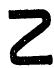
\includegraphics[keepaspectratio]{images/part002_bec1605a.jpg}}

一般说来，即使在波兰空间中，苏斯林子空间的余集也未必是苏斯林的（参看习题 6）；但参看第 6 号定理 2 的推论。

命题 9. 设 X 是可度量化空间，A 是 X 的相对紧苏斯林子空间。则存在一个紧可度量化空间 K 、K 的子集的一个递减序列 \((\mathbf{B}_{n})\) （其中每个子集都是紧集的可数并）以及一个连续映射 \(f: K \to X\) ，使得 \(A = f\left(\bigcap_{n} B_{n}\right)\) 。

必要时以 \(\overline{\mathbf{A}}\) 代替 X ，可设 X 是紧的且 A 在 X 中稠密。由于 A 是苏斯林空间，存在波兰空间 P 与连续映射 \(g: \mathrm{P} \to \mathrm{X}\) 使 \(g(\mathrm{P}) = \mathrm{A}\) 。由第 1 号定理 1 的推论 1 ，可设 P 是递减序列 \((\mathbf{U}_n)\) 的交，其中诸项是方体 \(\mathbf{I}^{\mathbf{N}}\) 的开子集。设 K 为空间 \(\mathbf{I}^{\mathbf{N}} \times \mathbf{X}\) ，它是紧且可度量化的（§ 2，第 4 号，定理 1 的推论 2）。设 \(\mathbf{G} \subset \mathbf{P} \times \mathbf{X}\) 是 \(g\) 的图像，\(\overline{\mathbf{G}}\) 是 G 在 K 中的闭包，而 \(f\) 表示 \(\mathbf{K} = \mathbf{I}^{\mathbf{N}} \times \mathbf{X}\) 到 X 上的投影；则显然有 \(f(\mathbf{G}) = \mathbf{A}\) 。由于 \(g\) 连续，G 在 \(\mathbf{P} \times \mathbf{X}\) 中闭（第 I 章，§ 8，第 1 号，命题 2 的推论 2），且 \(\mathbf{G} = \overline{\mathbf{G}} \cap (\mathbf{P} \times \mathbf{X})\) ；故 \(\mathbf{G} = \bigcap_{n=1}^{n} \mathbf{B}_n\) ，其中

\[
\mathbf {B} _ {n} = \overline {{\mathbf {G}}} \cap (\mathbf {U} _ {n} \times \mathbf {X}).
\]

由于每个 \(U_{n}\) 都是 \(I^{N}\) 中闭集的可数并（§ 2，第 5 号，命题 7），每个 \(B_{n}\) 都是紧集的可数并，证明完毕。

\subsection{波莱尔集}

定义 3. 设 X 是一个集，\(\mathfrak{X}\) 是 X 的子集所成的一个集。\(\mathfrak{X}\) 称为 X 上的一个 \(\sigma\) 代数，如果下列条件满足：

\begin{enumerate}
\def\labelenumi{\alph{enumi})}
\item
  \(\mathfrak{S}\) 中每个集的余集属于 \(\mathfrak{S}\) 。
\item
  \(\mathfrak{X}\) 中集合的每个可数交属于 \(\mathfrak{X}\) 。
\end{enumerate}

若 \(\mathfrak{X}\) 是一个 \(\sigma\) 代数（在 \(\mathbf{X}\) 上），则 \(\mathfrak{X}\) 中集合的每个可数并都属于 \(\mathfrak{X}\) （因为此并的余集是 \(\mathfrak{X}\) 中集合的交）。

X 的所有子集所成的集 \(\mathfrak{P}(\mathbf{X})\) 显然是一个 \(\sigma\) 代数。X 上的 \(\sigma\) 代数的每个交是 X 上的 \(\sigma\) 代数。因此，对 \(\mathfrak{P}(\mathbf{X})\) 的任意子集 F ，存在包含 F 的最小 \(\sigma\) 代数；它称为由 F 生成的 \(\sigma\) 代数。

定义 4. 在拓扑空间 X 中，由 X 的所有闭子集所成的集生成的 \(\sigma\) 代数的元素称为 X 中的波莱尔集。

命题 10. 设 \(f\) 是拓扑空间 \(\mathbf{X}\) 到拓扑空间 \(\mathbf{Y}\) 中的连续映射。则在 \(f\) 之下，\(\mathbf{Y}\) 中每个波莱尔集的原像是 \(\mathbf{X}\) 中的波莱尔集。

设 \(\mathfrak{X}\) 是满足如下条件的诸集 \(\mathbf{A}\) （ \(\mathbf{Y}\) 的子集）所成的集：\(\overline{f}^1 (\mathbf{A})\) 是 \(\mathbf{X}\) 中的波莱尔集。由此立得 \(\mathfrak{X}\) 是一个 \(\sigma\) 代数，它包含 \(\mathbf{Y}\) 的所有闭子集；从而 \(\mathfrak{X}\) 包含 \(\mathbf{Y}\) 中的所有波莱尔集。

命题 11. 在苏斯林空间 X 中，每个波莱尔集都是苏斯林集。

设 \(\mathfrak{X}\) 是由 X 的诸子集 A 中 A 与 CA 都是苏斯林集者所成的集。由第 2 号的命题 8 ，\(\mathfrak{X}\) 是一个 \(\sigma\) 代数。X 的每个闭子集 F 属于 \(\mathfrak{X}\) ，因为 F 与 CF 都是苏斯林集（第 2 号，命题 5）；从而 \(\mathfrak{X}\) 包含 X 的所有波莱尔集（参看第 6 号，定理 2 的推论）。

推论. 设 \(f\) 是苏斯林空间 \(\mathbf{X}\) 到可度量化空间 \(\mathbf{Y}\) 中的连续映射。若 \(\mathbf{B}\) 是 \(\mathbf{X}\) 中的任意波莱尔集，则 \(f(\mathbf{B})\) 是 \(\mathbf{Y}\) 中的苏斯林集。

因为 B 是苏斯林空间，故由定义 2 后的注（第 2 号），\(f(\mathbf{B})\) 也是苏斯林空间。

\pandocbounded{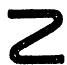
\includegraphics[keepaspectratio]{images/part002_bde2d1b5.jpg}}

注。1) 即使 X 与 Y 都是波兰空间，一般说来，X 中的波莱尔集在 X 到 Y 中的连续映射下的像未必是 Y 中的波莱尔集（参看习题 6；以及第 7 号，定理 3 的推论）。

\begin{enumerate}
\def\labelenumi{\arabic{enumi})}
\setcounter{enumi}{1}
\tightlist
\item
  设 X 是拓扑空间，Y 是 X 的波莱尔子集。则空间 Y 的波莱尔集恰是 X 的含于 Y 的那些波莱尔集。因为 (i) X 中含于 Y 的波莱尔集构成 Y 上的一个 σ 代数，它包含 Y 中的闭集，从而包含 Y 的所有波莱尔集；(ii) X 的使 A∩Y 是 Y 的波莱尔集的那些子集 A 构成 X 上的一个 σ 代数，它包含 X 的所有闭集，从而包含 X 的所有波莱尔集。
\end{enumerate}

\subsection{零维空间与卢津空间}

定义 5. 拓扑空间称为零维的，如果它是豪斯多夫的，且每个点有一个既开又闭的邻域基本系。

每个零维空间 X 都是全不连通的；因为一点的连通分支含于所有包含该点且既开又闭的集（第 I 章，§ 11，第 5 号），而这些集的交正是 \(\{x\}\) ，若 \(\mathbf{X}\) 是零维的。

反之，局部紧全不连通空间是零维的（第 II 章，§ 4，第 4 号，命题 6）；但存在不是零维的全不连通可度量化空间{[}习题 3 b){]}。

零维空间的每个子空间是零维的，且零维空间的拓扑和与积是零维的。

定义 6. 拓扑空间 X 是卢津空间，如果它可度量化，且存在一个零维波兰空间 P 和 P 到 X 上的连续双射映射。

显然每个卢津空间都是苏斯林空间。

命题 12. 可度量化空间是卢津空间，当且仅当它是一个波兰空间在连续双射映射下的像。

此条件显然必要；我们证明它也充分。若 f 是卢津空间 X 到可度量化空间 Y 上的连续双射，则由定义 6 ，Y 是卢津空间。故只需证明波兰空间是卢津空间。

首先注意，若 X 是卢津空间，则 X 的每个闭（相应地，开）子空间 A 是卢津空间（参看第 7 号，定理 3）；因为若 f 是零维波兰空间 P 到 X 上的连续双射，则 \(\overline{f}^{1}(A)\) 在 P 中闭（相应地，开），因而是 P 的零维波兰子空间（第 1 号，命题 1 与命题 2）。

卢津空间的每个可数积是卢津空间；这由第 1 号的命题 1 及零维空间的每个积是零维的这一事实得出。豪斯多夫拓扑空间中卢津子空间的每个可数交是卢津子空间；这由前面的注及第 1 号的引理 1 得出。此外：

引理 2. 若可度量化空间 X 使得存在 X 的一个由卢津子空间组成的可数分划 \((\mathbf{A}_{n})\) ，则 X 是卢津空间。

对每个 n ，设 \(P_{n}\) 是零维波兰空间，\(f_{n}\) 是 \(P_{n}\) 到 \(A_{n}\) 上的连续双射。若 P 是诸 \(P_{n}\) 的拓扑和，则 P 是波兰的（第 1 号，命题 1）且零维，而映射 \(f: P \to X\) （它与 \(f_{n}\) 在每个 \(P_{n}\) 上（对每个 n ）一致）是 P 到 X 上的连续双射；由此即得结论。

现在证明 R 的区间 \(I = [0, i]\) 是卢津空间。设 J 是由 I 中所有无理数组成的子空间；则 J 是波兰空间（第 1 号，命题 3 的推论）；且 J 是零维的，因为若 x 是 J 的任意点，则 R 中形如 {]}r, s{[} （其中 r 与 s 是有理数且 r \textless{} x \textless{} s ）的区间在 J 上的迹构成 x 在 J 中的既开又闭邻域的基本系（因为 {]}r, s{[} 与 {[}r, s{]} 在 J 上的迹相同）。故 J 是 I 的卢津子空间。而 J 与 I 的每个由单个有理点组成的子空间构成 I 的可数分划，因此由引理 2 ，I 是卢津空间。

设 P 是任意波兰空间。由定理 1 的推论 1 （第 1 号），P 同胚于方体 IN 的一个子空间，后者是 IN 中开集的可数交。由于 I 是卢津空间，证明开头的诸注表明 P 是卢津空间，从而命题 12 的证明完成。

\subsection{筛}

定义 7. 筛是一个序列 \(\mathbf{C} = (\mathbf{C}_n, p_n)_{n \geqslant 0}\) ，使得对每个 \(n\) ，\(\mathbf{C}_n\) 是可数集，而 \(p_n\) 是 \(\mathbf{C}_{n+1}\) 到 \(\mathbf{C}_n\) 上的满射。

对每对整数 \(m, n\) （满足 \(0 \leqslant m \leqslant n\) ），令 \(p_{mn}\) 表示 \(C_m\) 到自身的恒等映射（若 \(m = n\) ），或映射 \(p_m \circ p_{m+1} \circ \cdots \circ p_{n-1}\) （它是 \(C_n\) 到 \(C_m\) 上的满射，若 \(m < n\) ）。显然 \(p_{mq} = p_{mn} \circ p_{ng}\) 对 \(m \leqslant n \leqslant q\) 成立，因此可以考虑 \(L(C)\) ，即族 \((C_n)\) 关于映射族 \((p_{mn})\) 的逆极限（集合论，第 III 章，§ 7）。若每个 \(C_n\) 赋以离散拓扑，则 \(L(C)\) 是拓扑空间的逆极限（第 I 章，§ 4，第 4 号）；作为这样的空间，\(L(C)\) 称为与筛 \(C\) 相伴的拓扑空间。\(L(C)\) 是拓扑积 \(\prod_n C_n\) 的闭子空间，由此立得 \(L(C)\) 是零维波兰空间（第 4 号）。

度量空间 X 的一个筛分由一个筛 \(\mathbf{C} = (\mathbf{C}_{n}, p_{n})\) 以及对每个整数 \(n \geqslant 0\) 的一个映射 \(\varphi_{n}\) 组成，后者把 \(C_{n}\) 映到 X 的直径 \(\leqslant 2^{-n}\) 的非空闭子集所成的集中，且满足：

\begin{enumerate}
\def\labelenumi{\alph{enumi})}
\item
  X 是诸集 \(\varphi_0(c)\) （当 \(c\) 跑遍 \(\mathbf{C}_0\) ）的并；
\item
  对每个 \(n\) 与每个 \(c \in \mathbf{C}_n\) ，\(\varphi_n(c)\) 是诸集 \(\varphi_{n+1}(c')\) （其中 \(c'\) 跑遍 \(\overline{\pmb{p}}_n(c)\) ）的并。
\end{enumerate}

筛分称为严格筛分，如果此外对每个 n ，诸集 \(\varphi_{n}(c)\) （当 c 跑遍 \(C_{n}\) ）两两不相交。

引理 3. 每个可数型度量空间 X 都具有一个筛分。若 X 还是零维的，则 X 具有严格筛分。

首先注意，若 Y 是可数型度量空间，\(\varepsilon\) 是实数 \textgreater0 ，则存在 Y 的由直径 \(\leqslant\varepsilon\) 的集组成的可数覆盖（§2，第 8 号，命题 13）。此外，若 Y 是零维的，则存在这样的、由既开又闭的集组成的覆盖 \((\mathbf{V}_{n})\) ；若 \(W_{n}\) 是 \(V_{n}\) 与 \(\bigcap_{k<n}(\mathbf{Y}-\mathbf{V}_{k})\) 的交，则可见诸 \(W_{n}\) 是闭的、直径 \(\leqslant\varepsilon\) 、两两不相交且覆盖 X。无论如何，覆盖中非空集的闭包构成 Y 的一个可数覆盖，其元素是直径 \(\leqslant\varepsilon\) 的非空闭集。

设 X 是可数型度量空间。设 \(C_{0}\) 是 X 的一个由直径 \(\leqslant I\) 的非空闭集组成的可数覆盖的指标集（若 X 是零维的，这些集两两不相交）；\(\varphi_{0}\) 是使每个指标 \(c \in C_{0}\) 对应于覆盖中相应集的映射。设我们已定义了诸 \(C_{i}\) 、诸 \(\varphi_{i}\) 与满射映射 \(p_{i}: C_{i+1} \to C_{i}\) （对 \(i \leqslant n\) ），使得对这些指标条件 b) 满足。若 \(c \in C_{n}\) ，则空间 \(\varphi_{n}(c)\) 有一个由直径 \(\leqslant I/2^{n+1}\) 的非空闭集组成的可数覆盖（若 X {[}从而 \(\varphi_{n}(c)\) {]}是零维的，这些集两两不相交）；若 \(\mathrm{I}(c)\) 表示此覆盖的指标集，我们取 \(c_{n+1}\) 为诸集 \(\mathrm{I}(c)\) （当 c 跑遍 \(C_{n}\) ）之和；对每个 \(c' \in C_{n+1}\) ，令 \(p_{n}(c')\) 表示元素 \(c \in C_{n}\) 中满足 \(c' \in \mathrm{I}(c)\) 者，并令 \(\varphi_{n+1}(c')\) 表示指标为 \(c'\) 的集（在所考虑的 \(\varphi_{n}(c)\) 的覆盖中）。显然我们这样归纳地定义了 X 的一个筛分，且若 X 是零维的，此筛分是严格的；由此得引理 3 。

现在设 X 是可数型完备度量空间，考虑 X 的由一个筛 C 与诸映射 \(\varphi_{n}\) 给出的一个筛分。若 \(\gamma = (c_{n})\) 是与 C 相伴的空间 \(\mathrm{L}(\mathrm{C})\) 的一点，则序列 \((\varphi_{n}(c_{n}))\) 是 X 中闭集的递减序列，其直径趋于 0 ；因此这序列的集的交由单独一点组成，我们记之为 \(f(\gamma)\) 。这样我们就定义了一个映射 \(f: \mathrm{L}(\mathrm{C}) \to \mathrm{X}\) 。若 \(\gamma, \gamma'\) 是 \(\mathrm{L}(\mathrm{C})\) 的两点，它们对 \(i \leqslant n\) 有相同的第 i 坐标，则显然 \(f(\gamma)\) 与 \(f(\gamma')\) 之间的距离 \(\leqslant 1/2^{n}\) ，从而 f 是连续的（由 \(\mathrm{L}(\mathrm{C})\) 的拓扑的定义）。对每个 \(x \in X\) ，由筛分的定义可用对 n 的归纳定义一个序列 \(\gamma = (c_{n})\) ，使得 \(x \in \varphi_{n}(c_{n})\) 对每个 \(n \geqslant 0\) 成立，且 \(c_{n} = p_{n}(c_{n+1})\) ；因此 \(x = f(\gamma)\) ，故 f 是满射。此外，若筛分是严格的，则序列 \(\gamma = (c_{n})\) （它满足 \(x = f(\gamma)\) ）是唯一的，故在此情形 f 是双射。f 称为所考虑筛分诱导的映射。

命题 13. 若 X 是任意卢津（相应地，苏斯林）空间，则存在一个筛 C 与 L(C) 到 X 上的连续双射（相应地，满射）。

参照卢津空间的定义（第 4 号，定义 6）{[}相应地，苏斯林空间的定义（第 2 号，定义 2）{]}，我们归结到如下情形：

X 是零维波兰空间（相应地，波兰空间），而前面的论证随即证明此结果。

\subsection{苏斯林集的分离}

定理 2. 设 X 是可度量化空间。若给定 X 的两两不相交的苏斯林子空间的一个序列 \((\mathbf{X}_{n})\) ，则存在 X 中两两不相交的波莱尔集的一个序列 \((\mathbf{B}_{n})\) ，使得对每个 n 有 \(X_{n} \subset B_{n}\) 。

证明基于两个引理：

引理 4. 设 \((\mathbf{A}_n), (\mathbf{A}_m')\) 是拓扑空间 \(\mathbf{X}\) 的子集的两个序列。假设对每对 \((\mathbf{A}_n, \mathbf{A}_m')\) 有一个波莱尔集 \(\mathbf{B}_{nm}\) （ \(\mathbf{X}\) 中的），使得 \(\mathbf{B}_{nm} \supset \mathbf{A}_n\) 且 \(\mathbf{B}_{nm} \cap \mathbf{A}_m' = \emptyset\) 。则存在一个波莱尔集 \(\mathbf{B}\) （ \(\mathbf{X}\) 中的），它包含 \(\bigcup_{n} \mathbf{A}_n\) 且不交 \(\bigcup_{m} \mathbf{A}_m'\) 。

因为波莱尔集 \(\mathbf{B} = \bigcup_{n}\left(\bigcap_{m}\mathrm{B}_{nm}\right)\) 满足这些条件。

引理 5. 设 X 是豪斯多夫空间，A 、A' 是 X 的两个不相交的苏斯林子空间。则存在 X 的一个波莱尔集 B ，使得 B ⊃ A 且 B ∩ A' = ∅。

由第 5 号的命题 13 ，存在两个筛 \(\mathbf{C}\) 、\(\mathbf{C}'\) 与连续映射 \(f\) （ \(\mathbf{L}(\mathbf{C})\) 到 \(\mathbf{A}\) 上的）、\(f'\) （ \(\mathbf{L}(\mathbf{C}')\) 到 \(\mathbf{A}'\) 上的），它们用第 5 号中描述的方法构造。对每个 \(n \geqslant 0\) 与每个 \(c \in \mathbf{C}_n\) ，令 \(q_n(c)\) 表示 \(\mathbf{L}(\mathbf{C})\) 中由一切序列 \((c_k)_{k \geqslant 0}\) （满足 \(c_n = c\) 者）所成的子空间；\(q_n(c)\) 是 \(\mathbf{L}(\mathbf{C})\) 的闭子空间。对每个 \(\gamma = (c_n) \in \mathbf{L}(\mathbf{C})\) ，闭集序列 \(q_n(c_n)\) 是递减的，且构成以 \(\gamma\) 为极限的滤基。此外，对每个 \(c \in \mathbf{C}_n\) ，诸集 \(q_{n+1}(d)\) （其中 \(d\) 跑遍集 \(\overline{p_n}(c)\) ，此集在 \(\mathbf{C}_{n+1}\) 中）构成 \(q_n(c)\) 的一个分划。对筛 \(c'\) 作类似的记号定义。

我们将用反证法，假设每个包含 A 的波莱尔集都与 \(A'\) 相交。首先，由引理 4 与筛分的定义，存在 \(c_{0} \in C_{0}\) 与 \(c_{0}' \in C_{0}'\) ，使得每个包含 \(f(q_{0}(c_{0}))\) 的波莱尔集都与 \(f'(q_{0}'(c_{0}'))\) 相交。然后我们可以对 n 用归纳法定义

\[
\gamma = (c _ {n}) \in \mathrm{L} (\mathrm{C}) \quad \text { and } \quad \gamma^ {\prime} = (c _ {n} ^ {\prime}) \in \mathrm{L} (\mathrm{C} ^ {\prime})
\]

如下：设 \(c_i\) 与 \(c_i'\) 已对 \(i < n\) 定义，使得对每个指标 \(i < n\) ，每个包含 \(f(q_i(c_i))\) 的波莱尔集都与 \(f'(q_i'(c_i'))\) 相交；把引理 4 与筛分的定义应用于集 \(f(q_{n-1}(c_{n-1}))\) 与 \(f'(q_{n-1}'(c_{n-1}'))\) ，即见存在 \(c_n \in \mathbf{C}_n\) 与 \(c_n' \in \mathbf{C}_n'\) ，使得 \(p_{n-1}(c_n) = c_{n-1}\) 且 \(p_{n-1}(c_n') = c_{n-1}'\) 。

并使得每个包含 \(f(q_n(c_n))\) 的波莱尔集都与 \(f'(q_n'(c_n'))\) 相交。而序列 \(f(q_n(c_n))\) 收敛于一点 \(a = f(\gamma) \in \mathbf{A}\) ，序列 \(f'(q_n'(c_n'))\) 收敛于一点 \(a' = f'(\gamma') \in \mathbf{A}'\) 。由于 \(\mathbf{A} \cap \mathbf{A}' = \emptyset\) 且 \(\mathbf{X}\) 是豪斯多夫的，存在一个闭邻域 \(\mathbf{V}\) （ \(a\) 的），它不含 \(a'\) ，从而对充分大的 \(n\) ，\(\mathbf{V}\) 包含 \(f(q_n(c_n))\) 且不交 \(f'(q_n'(c_n'))\) 。这是矛盾，因为 \(\mathbf{V}\) 是波莱尔集。

为证定理 2 ，令 \(\mathbf{Y}_n\) 表示诸集 \(\mathbf{X}_i\) （满足 \(i \neq n\) 者）的并；则 \(\mathbf{Y}_n\) 是 \(\mathbf{X}\) 的苏斯林子空间（第 2 号，命题 8）。由引理 5 ，对每个指标 \(n\) 存在波莱尔集 \(\mathbf{B}_n'\) ，它包含 \(\mathbf{X}_n\) 且不交 \(\mathbf{Y}_n\) 。令 \(\mathbf{B}_n\) 为 \(\mathbf{B}_n'\) 与 \(\bigcap_{i < n} (\mathbf{X} - \mathbf{B}_i')\) 的交。则诸 \(\mathbf{B}_n\) 是波莱尔集，两两不相交，且 \(\mathbf{B}_n \supset \mathbf{X}_n\) 对每个 \(n\) 成立。

推论. 若可度量化空间的一个可数分划由苏斯林集组成，则这些集是波莱尔集。特别地，可度量化空间中余集为苏斯林集的每个苏斯林集是波莱尔集。

\subsection{卢津空间与波莱尔集}

定理 3. 设 X 是卢津空间。则 X 的子空间是卢津空间，当且仅当它是波莱尔集。

此定理是下述两个引理的推论：

引理 6. 在卢津空间 X 中，每个波莱尔集都是 X 的卢津子空间。

设 \(\mathfrak{X}\) 是由 X 的诸子集 A 中 A 与 \(\complement A\) 都是 X 的卢津子空间者所成的集。由于 X 中每个闭集与每个开集都是 X 的卢津子空间（第 4 号），\(\mathfrak{X}\) 包含 X 的所有闭子集，因此只要证明 \(\mathfrak{X}\) 是 X 上的一个 \(\sigma\) 代数，引理即得证。为此只需证明：若 \((A_n)\) 是 \(\mathfrak{X}\) 中集合的一个序列，则 \(\bigcap_{n} A_n\) 与 \(\bigcup_{n} A_n\) 都是 X 的卢津子空间。我们在第 4 号中已看到，卢津子空间的每个可数交是卢津子空间。另一方面，若 \(B_n\) 是 \(A_n\) 与 \(\bigcap_{i < n} \complement A_i\) 的交，则由假设与前面的注，\(B_n\) 是卢津子空间；且由于 \(\bigcup_{n} A_n = \bigcup_{n} B_n\) ，由第 4 号的引理 2 ，子空间 \(\bigcup_{n} A_n\) 是卢津子空间。

引理 7. 可度量化空间 X 的每个卢津子空间 A 都是 X 中的波莱尔集。

由第 5 号的命题 13 ，存在一个筛 C 与一个连续双射 \(f\) （ \(\mathbf{L}(\mathbf{C})\) 到 A 上的）。用第 6 号引理 5 的记号，对每个整数 \(n\) 与每个 \(c \in \mathbf{C}_n\) ，令 \(g_n(c)\) 表示 X 的子空间 \(f(q_n(c))\) ；它是卢津子空间，因而是 X 的苏斯林子空间。当 \(c\) 跑遍 \(\mathbf{C}_n\) 时，诸集 \(g_n(c)\) 两两不相交，因为 \(f\) 是双射；故由第 6 号的定理 2 ，存在 X 中波莱尔集的一个族 \(c \to g_n'(c) (c \in \mathbf{C}_n)\) ，两两不相交，且使 \(g_n'(c) \supset g_n(c)\) 对一切 \(c \in \mathbf{C}_n\) 成立。必要时以 \(g_n'(c)\) 与闭包 \(\overline{g_n(c)}\) （即 \(g_n(c)\) 在 X 中的闭包）的交代替之，可设 \(g_n'(c) \subset \overline{g_n(c)}\) 。令 \(c_{n-1}, c_{n-2}, \ldots, c_0\) 表示 \(c\) 在 \(\mathbf{C}_{n-1}, \mathbf{C}_{n-2}, \ldots, \mathbf{C}_0\) 中的像，所用满射为

\[
p _ {n - 1, n} = p _ {n - 1}, p _ {n - 2, n} = p _ {n - 2} \circ p _ {n - 1}, \dots , p _ {0 n} = p _ {0} \circ p _ {1} \circ \dots \circ p _ {n - 1}
\]

（分别为）；并令 \(h_n(c)\) 表示下列诸集

\[
g _ {n} ^ {\prime} (c), g _ {n - 1} ^ {\prime} \left(c _ {n - 1}\right), \dots , g _ {o} ^ {\prime} \left(c _ {0}\right).
\]

的交。由于 \(q_{i}(c_{i}) \supset q_{n}(c)\) 对 \(0 \leqslant i \leqslant n - 1\) 成立，\(h_{n}(c)\) 包含 \(g_{n}(c)\) ；同样显然 \(h_{n}(c)\) 是波莱尔集且含于 \(g_{n}(c)\) ，且当 \(c\) 跑遍 \(\mathbf{C}_{n}\) 时诸 \(h_{n}(c)\) 两两不相交；最后，由构造，对每个 \(c' \in \mathbf{C}_{n+1}\) 有 \(h_{n+1}(c') \subset h_n(p_n(c'))\) 。令 \(\mathbf{B}_n\) 为诸集 \(h_n(c)\) （当 \(c\) 跑遍 \(\mathbf{C}_n\) ）的并；\(\mathbf{B}_n\) 是波莱尔集，且 \(\mathbf{B}_{n+1} \subset \mathbf{B}_n\) ；又 \(\mathbf{B}_n\) 包含诸集 \(g_n(c) (c \in \mathbf{C}_n)\) 的并，即 A 。令 B 为递减集序列 \(\mathbf{B}_n\) 的交；B 是波莱尔集且包含 A 。我们将证明 B = A ，这样就完成了证明。

设 \(x\) 是 \(\mathbf{B}\) 的一点。则对每个整数 \(n\) ，存在唯一的 \(c \in \mathbf{C}_n\) 使 \(x \in h_n(c)\) ；我们把此 \(c\) 记作 \(c_n(x)\) 。序列 \((c_n(x))_{n \geqslant 0}\) 属于 \(\mathbf{L}(\mathbf{C})\) 。递减序列 \((g_n(c_n(x)))\) 依定义收敛于一点 \(a \in \mathbf{A}\) ；这些集的闭包序列也收敛于 \(a\) （在 \(\mathbf{X}\) 中），故序列 \((h_n(c_n(x)))\) 更加如此。而 \(x\) 属于所有集 \(h_n(c_n(x))\) ，因此 \(x = a \in \mathbf{A}\) 。引理 7 由此得证，定理 3 亦随之得证。

推论. 若 \(f\) 是卢津空间（特别地，波兰空间）\(\mathbf{X}\) 到可度量化空间 \(\mathbf{Y}\) 中的连续单射映射，则 \(f(\mathbf{X})\) 是 \(\mathbf{Y}\) 中的波莱尔集。

\subsection{波莱尔截面}

定理 4. 设 X 是波兰空间，R 是 X 上的一个等价关系，使得模 R 的等价类在 X 中闭，且 X 中每个闭集（关于 R ）的饱和集是波莱尔集。则存在 X 中的一个波莱尔集，它与每个等价类恰交于一点。

取 X 上与它的拓扑相容且使 X 完备的一个度量。由第 5 号的引理 3 ，存在 X 的一个筛分，由一个筛 \(\mathbf{C} = (\mathbf{C}_{n}, p_{n})\) 与一个映射序列 \((\varphi_{n})\) 定义。对每个 \(c \in C_{n}\) ，令 \(g_{n}(c)\) 为闭集 \(\varphi_{n}(c)\) 关于 R 的饱和集；由假设，\(g_{n}(c)\) 是 X 中的波莱尔集。

由于每个集 \(\mathbf{C}_n\) 可数，我们可以把每个 \(\mathbf{C}_n\) 线性排序，使得小于一个给定元素的元素之集有限。对每个 \(c \in \mathbf{C}_n\) ，我们定义一个集 \(h_n(c)\) ，用对 \(n\) 的归纳，如下。首先，对 \(c \in \mathbf{C}_0\) ，\(h_0(c)\) 是 \(\varphi_0(c)\) 与诸集 \(\mathbf{X} - g_0(c')\) （其中 \(c' \in \mathbf{C}_0\) 且 \(c' < c\) ）的交。对 \(c \in \mathbf{C}_{n+1}\) ，\(h_{n+1}(c)\) 是 \(\varphi_{n+1}(c)\) 、\(h_n(\mathbf{P}_n(c))\) 与诸集 \(\mathbf{X} - g_{n+1}(c')\) （对 \(c' \in \mathbf{C}_{n+1}\) ，\(p_n(c') = p_n(c)\) 且 \(c' < c\) ）的交。诸 \(h_n(c)\) 显然是波莱尔集。

我们将证明下述断言：对每个整数 \(n \geqslant 0\) 与每个等价类 \(\mathbf{H} \mod \mathbb{R}\) ，存在唯一的元素 \(c \in \mathbf{C}_n\) 使 \(h_n(c)\) 与 \(\mathbf{H}\) 相交，且我们有

\[
h (c _ {n}) \cap \mathrm{H} = \varphi_ {n} (c) \cap \mathrm{H},
\]

它因而是闭集。对 \(n = 0\) ，考虑最小的元素 \(c \in \mathbf{C}_0\) （使 \(\varphi_0(c)\) 与 \(\mathbf{H}\) 相交者）；则 \(\varphi_0(c) \cap \mathbf{H}\) 不交任何集 \(g_0(c')\) （对满足 \(c' \in \mathbf{C}_0\) 且 \(c' < c\) 的 c' ）；故它含于 \(h_0(c) \cap \mathbf{H}\) ，从而等于此集；此外，我们有 \(\mathbf{H} \subset g_0(c)\) ，因此 \(h_0(c') \cap \mathbf{H}\) 为空（对 \(c' \in \mathbf{C}_0\) 且 \(c' > c\) ）；这样断言对 \(n = 0\) 得证。我们对 \(n\) 继续用归纳法：若存在 \(c \in \mathbf{C}_{n+1}\) 使 \(h_{n+1}(c)\) 与 \(\mathbf{H}\) 相交，则由关系 \(h_{n+1}(c) \subset h_n(p_n(c))\) 与归纳假设，\(p_n(c)\) 是唯一的元素 \(d \in \mathbf{C}_n\) （使 \(h_n(d)\) 与 \(\mathbf{H}\) 相交者）。注意 \(h_n(d)\) 含于 \(\varphi_n(d)\) ，由筛分的定义，它含于诸集 \(\varphi_n(c)\) （对 \(c \in p_n(d)\) ）的并；因此存在最小元素 \(c \in p_n(d)\) 使 \(\varphi_{n+1}(c)\) 与 \(\mathbf{H}\) 相交。因此我们有

\[
\varphi_ {n + 1} (c) \cap \mathrm{H} \subset \varphi_ {n} (d) \cap \mathrm{H} = h _ {n} (d) \cap \mathrm{H}
\]

（依归纳假设）。从而

\[
\varphi_ {n + 1} (c) \cap \mathrm{H} \subset \varphi_ {n + 1} (c) \cap h _ {n} (d),
\]

且由于依定义 \(\varphi_{n+1}(c) \cap \mathbf{H}\) 不交任何集 \(g_{n+1}(c')\) （对满足 \(c' \in p_n(d)\) 且 \(c' < c\) 的 c' ），由 \(h_{n+1}(c)\) 的定义即得 \(\varphi_{n+1}(c) \cap \mathbf{H} = h_{n+1}(c) \cap \mathbf{H}\) 。此外，我们有 \(\mathbf{H} \subset g_{n+1}(c)\) ，因此若 \(c' \in p_n(d)\) 满足 \(c' > c\) ，则 \(h_{n+1}(c') \cap \mathbf{H}\) 为空。这样断言对一切 \(n\) 得证。

对每个整数 \(n\) ，令 \(\mathbf{S}_n\) 为诸集 \(h_n(c)\) （其中 \(c\) 跑遍 \(\mathbf{C}_n\) ）的并。集 \(\mathbf{S}_n\) 是波莱尔集，且我们有 \(\mathbf{S}_{n+1} \subset \mathbf{S}_n\) 。

令 S 为诸集 \(S_{n}\) 的交，它也是 X 中的波莱尔集；我们将证明 S 与每个等价类 H 模 R 恰交于一点。对每个 n ，令 \(c_{n}(H)\) 为唯一的元素 \(c \in C_{n}\) （使 \(h_{n}(c)\) 与 H 相交者）；则 \(\mathbf{S}_{n} \cap \mathbf{H} = \varphi_{n}(c_{n}(\mathbf{H})) \cap \mathbf{H}\) ，而 \(S \cap H\) 是诸集 \(\varphi_{n}(c_{n}(\mathbf{H})) \cap \mathbf{H}\) 的交。由于序列 \((c_{n}(\mathbf{H}))\) 属于 L(C)，闭集的递减序列 \(\varphi_{n}(c_{n}(\mathbf{H}))\) —— 其直径趋于 0 —— 收敛于一点 \(x \in X\) ，因为 X 完备。诸闭集 \(\varphi_{n}(c_{n}(\mathbf{H})) \cap \mathbf{H}\) 的交因此由单独一点 x 组成，定理 4 的证明完成。

注. 特别地，闭等价关系 R 满足定理 4 的假设。当 X 是紧可度量化空间时，定理 4 因此适用于任意豪斯多夫等价关系 R ，因为紧空间上的豪斯多夫等价关系是闭的（第 I 章，§ 10，第 4 号，命题 8）。

\subsection{苏斯林集的可容性}

定义 8. 设 X 是豪斯多夫拓扑空间。X 上的一个容度是 X 的所有子集所成的集 \(\mathfrak{P}(\mathbf{X})\) 到扩充实直线 \(\overline{\mathbf{R}}\) 中的一个映射 f ，满足下列条件：

\((\mathbf{CA}_{\mathbf{I}})\) 若 \(\mathbf{A} \subset \mathbf{B}\) ，则 \(f(\mathbf{A}) \leqslant f(\mathbf{B})\) 。

\((\mathbf{CA}_{\mathbf{II}})\) 若 \((\mathbf{A}_n)\) 是 \(\mathbf{X}\) 的子集的任意递增序列，则

\[
f \left(\bigcup_ {n} \mathrm{A} _ {n}\right) = \sup _ {n} f (\mathrm{A} _ {n}).
\]

\((\mathbf{CA}_{\mathbf{III}})\) 若 \((\mathbf{K}_n)\) 是 \(\mathbf{X}\) 的紧子集的任意递减序列，则

\[
f \left(\bigcap_ {n} \mathrm{K} _ {n}\right) = \inf _ {n} f (\mathrm{K} _ {n}).
\]

例。* 设 \(\mu\) 是局部紧空间 X 上的一个正测度；则对应的外测度 \(\mu^{*}\) 是 X 上的一个容度。可以证明，在欧氏空间 \(\mathbf{R}^{n}\) （ \(n \geqslant 3\) ）中，“牛顿外容度”是定义 8 意义下的容度。*

定义 9. 设 \(f\) 是 \(\mathbf{X}\) 上的一个容度；子集 \(\mathbf{A}\) （ \(\mathbf{X}\) 的）称为可容的（关于 \(f\) ），如果 \(f(\mathbf{A}) = \sup_k f(\mathbf{K})\) ，其中 \(\mathbf{K}\) 跑遍 \(\mathbf{A}\) 的紧子集所成的集。

* 例如，若 \(f\) 是一个外测度 \(\mu^{*}\) ，则每个开集都是可容的；满足 \(\mu^{*}(A) < +\infty\) 的可容集 A 恰是 \(\mu\) 可积集。*

命题 14. 设 K 是紧空间，f 是 K 上的一个容度。若 A 是 K 的子集的递减序列 \((\mathbf{A}_{n})\) 的交，其中每个子集都是闭集的可数并，则 A 是可容的。

只需证明，对每个 \(a < f(A)\) ，存在闭集 \(\mathbf{C} \subset \mathbf{A}\) 使 \(f(\mathbf{C}) \geqslant a\) 。首先证明存在闭集的一个序列 \((\mathbf{B}_n)_{n \geqslant 1}\) ，使得 \(\mathbf{B}_n \subset \mathbf{A}_n\) ，且使得序列 \((\mathbf{C}_n)\) 若由条件 \(\mathbf{C}_0 = \mathbf{A}\) 、\(\mathbf{C}_n = \mathbf{C}_{n-1} \cap \mathbf{B}_n\) （对 \(n \geqslant 1\) ）归纳地定义，则 \(f(\mathbf{C}_n) > a\) 对每个 \(n \geqslant 0\) 成立。设诸 \(\mathbf{B}_i\) 已对 \(i < n\) 定义；由假设我们有 \(\mathbf{C}_{n-1} \subset \mathbf{A} \subset \mathbf{A}_n\) 与 \(f(\mathbf{C}_{n-1}) > a\) ；由于 \(\mathbf{A}_n\) 是闭集的递增序列 \(\mathbf{D}_j\) 的并，由 \((\mathbf{CA}_{\mathbf{II}})\) 得

\[
f \left(\mathrm{C} _ {n - 1}\right) = \sup _ {j} f \left(\mathrm{C} _ {n - 1} \cap \mathrm{D} _ {j}\right).
\]

因此有一个指标 \(j\) 使 \(f(\mathbf{C}_{n-1} \cap \mathbf{D}_j) > a\) ，而我们可以取 \(\mathbf{B}_n = \mathbf{D}_j\) 。

现在令 \(\mathbf{C} = \bigcap_{n}\mathbf{C}_{n}\) 。由于 \(\mathbf{A} = \bigcap_{n}\mathbf{A}_{n}\) 且 \(\mathbf{B}_n\subset \mathbf{A}_n\) ，我们有

\[
\mathrm{C} = \bigcap_ {n} \mathrm{B} _ {n};
\]

因此集 C 是紧的且含于 A 。

令 \(B_n' = B_1 \cap B_2 \cap \cdots \cap B_n\) ；\((B_n')\) 是 K 的紧子集的递减序列；由于 \(C_n \subset C_i \subset B_i\) 对 i \textless{} n 成立，我们也有 \(C_n \subset B_n'\) 。由 \((CA_{III})\) ，\(f(C) = \inf_{n} f(B_n')\) ，且由于 \(C \subset C_n \subset B_n'\) 我们也有 \(f(C) = \inf_{n} f(C_n) \geqslant a\) 。这就完成了证明。

定理 5. 设 X 是可度量化空间，Y 是 X 的相对紧苏斯林子空间。则 Y 关于 X 上的每个容度 f 都是可容的。

我们已看到（第 2 号，命题 9），存在一个紧空间 K 、K 的子集的递减序列 \((\mathbf{A}_{n})\) （其中每个子集都是紧集的可数并）与一个连续映射 \(\varphi: K \to X\) ，使得 \(Y = \varphi\left(\bigcap_{n} A_{n}\right)\) 。由命题 14 ，\(\bigcap_{n} A_{n}\) 关于 K 上的每个容度都是可容的。因此定理 5 是下述命题的推论：

命题 15. 设 \(\varphi\) 是豪斯多夫空间 K 到豪斯多夫空间 X 中的连续映射，\(f\) 是 X 上的一个容度。若对 K 的每个子集 A 令 \(g(A) = f(\varphi(A))\) ，则 \(g\) 是 K 上的一个容度；此外，若 A 关于 \(g\) 是可容的，则 \(\varphi(A)\) 关于 \(f\) 是可容的。

显然 \(g\) 满足公理 \((\mathbf{CA}_{\mathbf{I}})\) 与 \((\mathbf{CA}_{\mathbf{II}})\) 。另一方面，设 \((\mathbf{C}_n)\) 是 \(\mathbf{K}\) 的紧子集的递减序列，并令 \(\mathbf{C} = \bigcap_{n} \mathbf{C}_n\) ；诸集 \(\varphi(\mathbf{C})\) 是紧的，它们的交是 \(\varphi(\mathbf{C})\) ；因为此交当然包含 \(\varphi(\mathbf{C})\) ，且若 \(x \in \varphi(\mathbf{C}_n)\) 对一切 \(n\) 成立，则诸集 \(\overline{\varphi}^1(x) \cap \mathbf{C}_n\) 构成 \(\mathbf{K}\) 的非空紧子集的递减序列，因此它们的交非空。于是我们有 \(f(\varphi(\mathbf{C})) = \inf_{n} f(\varphi(\mathbf{C}_n))\) ，即 \(g(\mathbf{C}) = \inf_{n} g(\mathbf{C}_n)\) ；这样 \(g\) 满足公理 \((\mathbf{CA}_{\mathbf{III}})\) ，因而是 \(\mathbf{K}\) 上的一个容度。

现在设 A 是 K 的关于 g 可容的子集；若 \(a < f(\varphi(A)) = g(A)\) ，则存在紧集 \(C \subset A\) 使 \(g(C) \geqslant a\) ；这样 \(\varphi(C)\) 是含于 \(\varphi(A)\) 的紧集，且 \(f(\varphi(C)) \geqslant a\) 。这表明 \(\varphi(A)\) 关于 f 是可容的，并完成了命题 15 从而定理 5 的证明。

注. * 若 \(\mu\) 是局部紧可度量化空间 X 上的一个正测度，则 X 的每个苏斯林子集 A 都是 \(\mu\) 可测的。因为若 K 是 X 的任意紧子集，则 K∩A 是相对紧苏斯林集，从而关于 \(\mu^{*}\) 是可容的，因而是 \(\mu\) 可积的。注意苏斯林集在 X 中的余集虽然一般不是苏斯林集，却是 \(\mu\) 可测的 *。

\appendix
\setcounter{chapter}{9}
\renewcommand{\thechapter}{\Roman{chapter}}
\setcounter{subsection}{0}
\renewcommand{\thesubsection}{\arabic{subsection}}

\section*{附录：赋范代数中的无穷乘积}
\phantomsection
\addcontentsline{toc}{section}{附录：赋范代数中的无穷乘积}

\subsection{赋范代数中的可乘序列}

设 A 是非离散赋值域 K 上的一个赋范代数（第 IX 章，§ 3，第 7 号，定义 9）；我们用 \(||x||\) 表示元素 \(x \in A\) 的范数，并设此范数满足不等式 \(||xy|| \leqslant ||x|| \cdot ||y||\) ；又设 A 有单位元 \(e\) 。设 \((x_n)_{n \in \mathbb{N}}\) 是 A 的点的一个无穷序列。N 的每个有限子集 J （以 N 的序线性排序）定义 A 的点的一个序列 \((x_n)_{n \in J}\) ，而我们定义积

\[
p _ {J} = \prod_ {n \in J} x _ {n}
\]

为此序列的积；此积称为序列 \((\pmb{x}_n)_{n\in \mathbb{N}}\) 的对应于有限子集 \(J\) （ \(\mathbb{N}\) 的）的有限部分积（回忆若 \(J = \emptyset\) ，我们令 \(\prod_{n\in \emptyset}x_n = e\) ）。

定义 1. 序列 \((\pmb{x}_n)_{n\in \mathbb{N}}\) 称为在赋范代数 \(\mathbf{A}\) 中可乘的，如果映射 \(\mathbf{J}\to \pmb{p}_{\mathbf{J}}\) 关于有限子集所成的集 \(\mathfrak{F}(\mathbf{N})\) （ \(\mathbf{N}\) 的）的截口滤有极限，此集以关系 \(c\) 排序；此极限称为序列 \((\pmb{x}_n)_{n\in \mathbb{N}}\) 的积，记作 \(\prod_{n\in \mathbb{N}}\pmb{x}_n\) （或简作 \(\prod_{n}\pmb{x}_n\) ）；诸 \(\pmb{x}_n\) 称为此积的因子。

定义 1 等价于下述：序列 \((\pmb{x}_n)\) 可乘且其积为 \(\pmb{p}\) ，如果对每个 \(\varepsilon > 0\) 存在有限子集 \(J_0\) （ \(\mathbf{N}\) 的），使得对每个有限子集 \(J \supset J_0\) （ \(\mathbf{N}\) 的），有 \(||\pmb{p}_{\mathrm{J}} - \pmb{p}|| \leqslant \varepsilon\) 。

注。1) 当 A 是交换代数时，定义 1 与第 III 章，§ 5，第 1 号，注 3 中所给的相同；但当 A 不交换时，指标集 N 的序结构本质上涉及定义 1 。若 \(\sigma\) 是 N 的任意置换，一般不能断言序列 \((\pmb{x}_{\sigma(n)})\) 在序列 \((x_{n})\) 可乘时可乘；且若两个序列都可乘，它们的积一般不同。

\begin{enumerate}
\def\labelenumi{\arabic{enumi})}
\setcounter{enumi}{1}
\tightlist
\item
  定义 1 可以直接推广到族 \((\pmb{x}_n)_{n\in I}\) 的情形，其指标集 I 是 \(\mathbf{Z}\) 的子集（以 \(\mathbf{Z}\) 的序所诱导的序线性排序）。我们将下述结果向此情形的推广留给读者（参看习题 1 与习题 2）。
\end{enumerate}

\subsection{可乘性判别法}

以下我们恒设赋范代数 A 是完备的。

定理 1. 设 \((\pmb{x}_n)_{n\in \mathbb{N}}\) 是完备赋范代数 A 中的点的一个序列。a) 若 \((\pmb{x}_n)\) 可乘且其积是 A 的一个单位，则对每个 \(\varepsilon >0\) 存在 N 的有限子集 \(\mathbf{J}_0\) ，使得对 N 的每个不交 \(\mathbf{J}_0\) 的有限子集 L ，有 \(||e - p_{\mathrm{L}}||\leqslant \varepsilon\) 。

\begin{enumerate}
\def\labelenumi{\alph{enumi})}
\setcounter{enumi}{1}
\item
  反之，若序列 \((\pmb{x}_n)\) 满足此条件，则它可乘。此外，若每个 \(\pmb{x}_n\) 是单位，则 \(\prod_{n\in \mathbb{N}}\pmb{x}_n\) 是单位。
\end{enumerate}

a) 设 \(\pmb{p}\) 是可乘序列 \((\pmb{x}_n)\) 的积，且设 \(\pmb{p}\) 是 A 中的单位；则（第 IX 章，§ 3，第 7 号，命题 13）存在 \(\alpha > 0\) 与 \(a > 0\) ，使得对一切满足如下条件的 \(y \in A\) ：

\[
\left| \left| \boldsymbol {y} - \boldsymbol {p} \right| \right| \leqslant \alpha ,
\]

y 是单位且 \(\|y^{-1}\|\leqslant a\) 。由假设，对每个 \(\varepsilon\) （满足 \(o<\varepsilon<\alpha\) ），存在 N 的有限子集 \(H_{0}\) ，使得对 N 的每个包含 \(H_{0}\) 的有限子集 H ，有 \(\|p_{H}-p\|\leqslant\varepsilon\) 。设 \(J_{0}=[0,m]\) 是包含 \(H_{0}\) 的 N 的一个区间；对 N 的每个不交 \(J_{0}\) 的有限子集 L ，属于 L 的整数都大于属于 \(H_{0}\) 的整数；因此，若 \(H=H_{0}\cup L\) ，我们有 \(p_{H}=p_{H_{0}}p_{L}\) 。现在，由于 \(\|p_{H_{0}}-p\|\leqslant\varepsilon\leqslant\alpha\) ，\(p_{H_{0}}\) 是单位，且

\[
\left| \left| e - p _ {\mathrm{H} _ {0}} ^ {- 1} p \right| \right| \leqslant \varepsilon \left| \left| p _ {\mathrm{H} _ {0}} ^ {- 1} p \right| \right| \leqslant a \varepsilon ;
\]

由于 \(||p_{\mathrm{H_0}}p_{\mathrm{L}} - p|| \leqslant \varepsilon\) ，我们推出

\[
\left| \left| p _ {\mathrm{L}} - p _ {\mathrm{H} _ {0}} ^ {- 1} p \right| \right| \leqslant \varepsilon \left| \left| p _ {\mathrm{H} _ {0}} ^ {- 1} \right| \right| \leqslant a \varepsilon ,
\]

而最终 \(||e - p_{\mathrm{L}}|| \leqslant 2a\varepsilon\) 。

\begin{enumerate}
\def\labelenumi{\alph{enumi})}
\setcounter{enumi}{1}
\tightlist
\item
  设对每个 \(\varepsilon > 0\) ，存在有限子集 \(J_0\) （ \(\mathbf{N}\) 的），使得对每个有限子集 \(\mathbf{L}\) （ \(\mathbf{N}\) 的，不交 \(J_0\) ），有 \(\|e - p_{\mathbf{L}}\| \leqslant \varepsilon\) 。设 \(H_0 = [0, p]\) 是 \(\mathbf{N}\) 的一个包含 \(J_0\) 的区间；则每个有限子集 \(\mathbf{H}\) （ \(\mathbf{N}\) 的，包含 \(H_0\) ）可写成 \(H_0 \cup L\) 的形式，其中 \(\mathbf{L}\) 中的整数都大于 \(H_0\) 中的整数；因此我们有 \(p_H = p_{H_0}p_L\) ，且由于 \(\mathbf{L}\) 不交 \(J_0\) ，\(||p_H - p_{H_0}|| \leqslant \varepsilon ||p_{H_0}||\) ，从而 \(||p_H|| = (1 + \varepsilon)||p_{H_0}||\) 。若 \(p_{H_0} = 0\) ，则序列 \((x_n)\) 显然可乘且其积为 0 ；除去这一平凡情形，存在区间 \(H_1 = [0, q]\) （它包含 \(H_0\) ），使得对 N 的每个不交 \(H_1\) 的有限子集 L ，有 \(||e - p_L|| \leqslant \varepsilon (||p_{H_0}||)^{-1}\) 。如上可得，对每个有限子集 \(H \supset H_1\) ，
\end{enumerate}

\[
\left| \left| p _ {\mathrm{H}} - p _ {\mathrm{H} _ {4}} \right| \right| \leqslant \left(\left| \left| p _ {\mathrm{H} _ {0}} \right| \right|\right) ^ {- 1} \left| \left| p _ {\mathrm{H} _ {4}} \right| \right| \varepsilon \leqslant \varepsilon (\mathrm{I} + \varepsilon).
\]

因此柯西判别法表明 \(J \to p_J\) 在 \(A\) 中（关于有序集 \(\mathfrak{F}(N)\) ）有极限。

若所有 \(x_{n}\) 都是单位，则所有有限部分积 \(p_{J}\) 也是单位；从而对每个包含 \(H_{0}\) 的有限子集 H ，我们有

\[
\left| \left| e - p _ {\mathrm{H} _ {0}} ^ {- 1} p _ {\mathrm{H}} \right| \right| \leqslant \varepsilon ,
\]

这表明，在 A 的单位所成的乘法群 G 中，映射 \(J \rightarrow p_{J}\) 下 \(\mathfrak{F}(N)\) 的截口滤的像是关于 G 的左一致结构的一个柯西滤基；但由于 G 完备（第 IX 章，§ 3，第 7 号，命题 13），映射 \(J \rightarrow p_{J}\) 的极限属于 G 。

注. 若 \((\pmb{x}_n)\) 可乘而其积不是单位，定理 1 的条件未必满足：例如，若所有 \(x_n\) 都等于同一元素 \(x\) ，其中 \(||x|| < 1\) ，则序列 \((\pmb{x}_n)\) 可乘且其积为 0 ，而对 N 的每个非空有限子集 H ，有 \(\| p_{\mathbf{H}} \| \leqslant \| x \| < 1 \leqslant \| e \|\) 。

推论 1. 若 \((\pmb{x}_n)\) 是积为 A 的单位的可乘序列，则 \(\lim_{n\to \infty}\pmb{x}_n = \pmb{e}\) 。

推论 2. 若 \((\pmb{x}_n)\) 是积为 A 的单位的可乘序列，则它的每个子序列 \((\pmb{x}_{n_k})_{k\in \mathbb{N}}\) （ \((\pmb{x}_n)[(n_k)\) 为严格递增的整数序列{]}）都是可乘的。

这由定理 1 的判别法立得。

定理 2. 设 A 是完备赋范代数。若 \((\pmb{u}_n)\) 是 A 的元素的一个绝对收敛级数，则序列 \((\pmb{e} + \pmb{u}_n)\) 在 A 中可乘；且若所有元素 \(\pmb{e} + \pmb{u}_n\) 都是 A 中的单位，则 \(\prod_{n\in \mathbb{N}}(\pmb {e} + \pmb{u}_n)\) 也是单位。

我们应用定理 1 的判别法。对 N 的每个有限子集 L ，有 \(p_{L} - e = \prod_{n \in L} (e + u_n) - e = \sum_{M} \left( \prod_{n \in M} u_n \right)\) ，其中 M 跑遍 L 的所有非空子集所成的集（以诱导的序线性排序）。由于 \(\left\| \prod_{n\in \mathbf{M}}\pmb {u}_n\right\| \leqslant \prod_{n\in \mathbf{M}}||\pmb {u}_n||,\) 我们可以写

\[
\left| \left| \boldsymbol {p} _ {\mathrm{L}} - \boldsymbol {e} \right| \right| \leqslant \sum_ {\mathbf {M}} \left(\prod_ {n \in \mathbf {M}} \left| \left| \boldsymbol {u} _ {n} \right|\right)\right) = \prod_ {n \in \mathbf {L}} (\mathrm{I} + \left| \left| \boldsymbol {u} _ {n} \right|\right) - \mathrm{I}.
\]

现在由于通项为 \(||\boldsymbol{u}_n||\) 的级数依假设收敛，序列 \((\mathbf{I} + ||\boldsymbol{u}_n||)\) 在 \(\mathbf{R}_+^*\) 中可乘（第 IV 章，§ 7，第 4 号，定理 4）。因此对每个 \(\varepsilon > 0\) 存在有限子集 \(J_0\) （ \(\mathbf{N}\) 的），使得对每个有限子集 \(\mathbf{L}\) （ \(\mathbf{N}\) 的，不交 \(J_0\) ），有 \(\left| \prod_{n \in \mathbf{L}} (\mathbf{I} + ||\boldsymbol{u}_n||) - \mathbf{I} \right| \leqslant \varepsilon\) ；由此即得结论。

推论. 若通项为 \(u_{n}\) 的级数绝对收敛，且诸元素 \(e + u_{n}\) 都不是 A 中的零因子，则积 \(\prod_{n \in \mathbb{N}} (e + u_{n})\) 不是 A 中的零因子。

只有有限个整数 \(n\) 满足 \(||\boldsymbol{u}_n|| \geqslant 1\) 。设 \(J = [0, m]\) 是 \(N\) 的一个包含所有这些整数的区间。序列 \((\boldsymbol{e} + \boldsymbol{u}_n)\) 的积是 \(p_J\) 与元素 \(\prod_{n > m} (\boldsymbol{e} + \boldsymbol{u}_n)\) 的积，后者的所有因子都是单位（第 IX 章，§ 3，第 7 号，命题 12 的推论），因而它本身是单位；由于 \(p_J\) 是有限个非零因子的积，它不是零因子，因此 \(\prod_{n \in N} (\boldsymbol{e} + \boldsymbol{u}_n)\) 不是零因子。

定理 2 给出的可乘性充分条件一般不是必要的（参看习题 6）。然而，在 A 是域 R 上有限秩代数（即 A 作为 R 上的向量空间是有限维的）这一重要情形中它是必要的；特别地，若 A 是四元数体 H 或矩阵代数 \(\mathbf{M}_n(\mathbf{R})\) ，就是这种情形：

命题 1. 设 A 是 R 上的有限秩赋范代数。若 \((\boldsymbol{e} + \boldsymbol{u}_{n})\) 是 A 中的可乘序列，其积是 A 的单位，则通项为 \(u_{n}\) 的级数绝对收敛。

由第 VII 章，§ 3，第 1 号，命题 2 ，存在数 \(c > 0\) ，使得对每个有限族 \((\pmb{x}_i)_{i \in \mathbf{I}}\) （ \(\mathbf{A}\) 的点组成的），我们有

\[
\sum_ {i \in \mathbf {I}} | | \boldsymbol {x} _ {i} | | \leqslant c. \sup _ {\mathrm{J} \subset \mathbf {I}} \left\| \sum_ {i \in \mathrm{J}} \boldsymbol {x} _ {i} \right\|.\tag{1}
\]

设 \((\pmb{a}_n)_{n\in \mathbb{N}}\) 是 A 的元素的任意序列。对 N 的每个有限子集 I ，令

\[
\boldsymbol {p} _ {\mathbf {I}} = \prod_ {i \in \mathbf {I}} (\boldsymbol {e} + \boldsymbol {a} _ {i}), \quad s _ {\mathbf {I}} = \sum_ {i \in \mathbf {I}} \boldsymbol {a} _ {i}, \quad \sigma_ {\mathbf {I}} = \sum_ {i \in \mathbf {I}} | | \boldsymbol {a} _ {i} | |.
\]

引理 1. 对 N 的每个有限子集 I ，令 \(\varphi(\mathrm{I}) = \sup_{\mathrm{J} \subset \mathrm{I}} ||\boldsymbol{p}_{\mathrm{J}} - \boldsymbol{e}||\) 。则对 I 的每个子集 J 我们有

\[
\left| \left| p _ {J} - e - s _ {J} \right| \right| \leqslant \varphi (I) \sigma_ {J}.\tag{2}
\]

若 \(J\) 为空则引理显然；我们对 \(J\) 的元素个数用归纳法证明。设 \(J = K \cup \{j\}\) ，其中 \(\{j\}\) 严格大于每个 \(i \in K\) 。则 \(p_J = p_K(e + a_j)\) 且

\[
s _ {\mathrm{J}} = s _ {\mathrm{K}} + a _ {j},
\]

从而

\[
p _ {J} - e - s _ {J} = p _ {K} - e - s _ {K} + (p _ {K} - e) a _ {j},
\]

而由归纳假设与 \(\varphi(\mathbf{I})\) 的定义，我们有

\[
\left| \left| p _ {J} - e - s _ {J} \right| \right| \leqslant \varphi (I) \sigma_ {K} + \varphi (I) \left| \left| a _ {j} \right| \right| = \varphi (I) \sigma_ {J},
\]

这就证明了引理。

引理 2. 若 I 是 N 的有限子集，满足 \(\varphi(\mathbf{I}) < \mathbf{i}/c\) ，则

\[
\sigma_ {\mathbf {I}} \leqslant c _ {\varphi} (\mathbf {I}) / (\mathbf {I} - c _ {\varphi} (\mathbf {I})).
\]

因为 \(\sigma_{\mathbf{J}} \leqslant \sigma_{\mathbf{I}}\) 对每个子集 \(J\) （ \(I\) 的）成立，由 (2) 得

\[
\left| \left| s _ {J} \right| \right| \leqslant \varphi (I) \sigma_ {I} + \left| \left| p _ {J} - e \right| \right| \leqslant (I + \sigma_ {I}) \varphi (I);
\]

又由于 \(\sigma_{\mathbf{I}} \leqslant c.\sup_{\mathbf{J} \in \mathbf{I}} ||s_{\mathbf{J}}||\) （由 (1) ），可得

\[
\sigma_ {\mathbf {I}} \leqslant c \varphi (\mathbf {I}) (\mathbf {I} + \sigma_ {\mathbf {I}}),
\]

由此即得结果。

现在设 \((e + u_{n})\) 是 A 中的可乘序列，其积为单位；由定理 1 存在 N 的有限子集 \(J_{0}\) ，使得对 N 的每个不交 \(J_{0}\) 的有限子集 H ，我们有

\[
\left\| \prod_ {i \in \mathbf {H}} (e + u _ {i}) - e \right\| \leqslant 1 / 2 c.
\]

由引理 2 得 \(\sum_{i\in\mathbf{H}}||\boldsymbol{u}_{i}||-\mathrm{i}\) （对 N 的每个不交 \(J_{0}\) 的有限子集 H ），从而（第 IV 章，§ 7，第 1 号，定理 1）族 \((||\boldsymbol{u}_{n}||)\) 在 R 中可和。

\subsection{无穷乘积}

对赋范代数 A 中的点的每个序列 \((\pmb{x}_n)\) ，使它对应于部分积的序列 \(p_n = \prod_{k=0}^{n} x_k\) ；则序列偶 \((x_{n})\) 与 \((p_{n})\) 称为以 \(x_{n}\) 为通项因子的无穷乘积。以 \(x_{n}\) 为通项因子的无穷乘积称为收敛的，如果序列 \((p_{n})\) 在 A 中收敛；此序列的极限则称为序列 \((x_{n})\) 的积，记作 \(\bigoplus_{n=0}^{\infty} x_{n}\) 。

命题 2. 设 \((\pmb{x}_n)\) 是完备赋范代数 A 中的点的一个序列。a) 若以 \(\pmb{x}_n\) 为通项因子的无穷乘积收敛，且 \(\mathbf{P}_{n=0}^{\infty}\pmb{x}_n\) 是 A 中的单位，则对每个 \(\varepsilon > 0\) 存在一个整数 \(n_0\) ，使得

\[
\left\| \prod_ {k = m} ^ {n} x _ {k} - e \right\| \leqslant \varepsilon
\]

每当 \(n_0 \leqslant m \leqslant n\) 。

\begin{enumerate}
\def\labelenumi{\alph{enumi})}
\setcounter{enumi}{1}
\tightlist
\item
  反之，若序列 \((\pmb{x}_n)\) 满足此条件，则以 \(\pmb{x}_n\) 为通项因子的无穷乘积收敛；且若每个 \(\pmb{x}_n\) 都是 A 中的单位，则 \(\mathbf{P}_{n=0}^{\infty}\pmb{x}_n\) 是单位。
\end{enumerate}

此命题的证明逐步仿照定理 1 的证明，留给读者（定理 1 证明中 N 的有限子集 L 应换成区间）。

推论 1. 若以 \(x_{n}\) 为通项因子的无穷乘积收敛，且 \(\bigcap_{n=0}^{\infty}x_{n}\) 是单位，则 \(\lim_{n\to\infty}x_{n}=e\) 。

推论 2. 若以 \(\pmb{x}_n\) 为通项因子的无穷乘积收敛，且 \(\mathop{\sum }\limits_{{n = 0}}^{\infty}{\pmb{x}}_{n}\) 是单位，则以

\[
\mathbf {y} _ {n} = \mathbf {x} _ {n + h} \quad (n \geqslant 0)
\]

为通项因子的无穷乘积收敛。

序列 \((\mathbf{y}_n)\) 的积记作 \(\bigoplus_{n = h}^{\infty}\mathbf{x}_n\) ，也称为无穷乘积的指标 \(h\) 的剩余，该无穷乘积以 \(\mathbf{x}_n\) 为通项因子。

仍在 \(\mathbf{P}_{n=h} x_n\) 是单位的假设下，由命题 2 得：若 \((z_n)\) 是一个序列，使得除去有限个指标外 \(z_n = x_n\) ，则以 \(z_n\) 为通项因子的乘积收敛。

命题 3. 设 \((k_{n})\) 是整数的一个严格递增序列，其项 \(\geqslant 0\) ，且满足 \(k_{0} = 0\) ；若以 \(x_{n}\) 为通项因子的无穷乘积收敛，且

若令

\[
\boldsymbol {u} _ {n} = \prod_ {p = k _ {n}} ^ {k _ {n + 1} - 1} \boldsymbol {x} _ {p},
\]

则以 \(u_{n}\) 为通项因子的无穷乘积收敛，且我们有

\[
\underset {n = 0} {\overset {\infty} {\mathsf {P}}} u _ {n} = \underset {n = 0} {\overset {\infty} {\mathsf {P}}} x _ {n}.
\]

因为序列 \((\boldsymbol{u}_{n})\) 的部分积序列是序列 \((\boldsymbol{x}_{n})\) 的部分积序列的一个子序列。

最后，对阿贝尔群用过的同样论证（第 III 章，§ 5，第 7 号）表明，若一个序列 \((\pmb{x}_n)\) （赋范代数 \(\mathbf{A}\) 中的）可乘，则以 \(\pmb{x}_n\) 为通项因子的乘积收敛，且

\[
\mathop {\text { P }} _ {n = 0} ^ {\infty} x _ {n} = \prod_ {n \in \mathbf {N}} x _ {n}
\]

（它也写作 \(\prod_{n=0}^{\infty} x_n\) ）；反之当然不真（参看习题 7）。
